%!TEX TS-program = xelatex
% Much of the initial version of this lab manual was taken from Jonathan Peelle's lab manual. 
% See original source here: https://github.com/jpeelle/peellelab_manual/

\documentclass[letterpaper,11pt,oneside]{memoir}
\usepackage{color}

%\setromanfont{Cambria}
\usepackage{xunicode,fontspec,xltxtra} 
\usepackage{libertine} 

\usepackage[pdftitle={Smith Lab Manual}, pdfauthor={David V. Smith}, colorlinks=true, urlcolor=blue]{hyperref}

\usepackage{multicol}
\usepackage{array,ragged2e}
\usepackage{fontspec,xunicode}
\defaultfontfeatures{Mapping=tex-text}

\definecolor{shadecolor}{gray}{0.9}
\setsecnumdepth{section}
\maxtocdepth{subsection}
\usepackage{multicol}
\usepackage{enumitem}

\usepackage{xurl}

\renewcommand{\UrlFont}{\ttfamily\footnotesize}

\chapterstyle{article}



%\pretitle{\huge\sffamily}
%\posttitle{\vskip 0.5em}
% \preauthor{\begin{flushleft}}
%\postauthor{\end{flushleft}}
%\predate{\begin{flushleft}}
 %\postdate{\end{flushleft}}

\setlength{\droptitle}{1in}

\checkandfixthelayout	% for memoir class

\begin{document}

\title{Smith Lab Manual}
\author{David V. Smith\\Department of Psychology\\Temple University}
\date{\today}

%\href{https://sites.google.com/a/temple.edu/dvs-lab/SmithLab\_manual.pdf}{Link to Lab Manual}

\maketitle

\pagestyle{titlingpage}


\cleardoublepage
\frontmatter
\tableofcontents
\cleardoublepage

\mainmatter

\pagestyle{headings}

%%%%%%%%%%%%%%%%%%%%%
\chapter{Introduction}

My overarching goal is to foster an environment of scientific excellence and personal development for all lab members. We should continually strive to learn and improve---and we should also try to have fun doing great science. This Lab Manual\footnote{Much of this document is derived from Dr. Jonathan Peelle's excellent \href{https://github.com/jpeelle/peellelab\_manual/}{Lab Manual}.} is meant to be the first resource for the lab as we seek to achieve these goals. You can also find the lab elsewhere:

\begin{itemize}[noitemsep]
\item Website: \url{https://sites.temple.edu/neuroeconlab/}
\item GitHub: \url{https://github.com/DVS-Lab}
\item Twitter: \url{https://twitter.com/DVSneuro}
% \item Mendeley: \url{https://www.mendeley.com/community/smith-lab-meetings/} 
\item OSF: \url{https://osf.io/5zq6h/} \footnotesize{[we are working on a better system for using OSF]}
\end{itemize}

\noindent There are also a couple of sites accessible only by lab members:

\begin{itemize}[noitemsep]
\item Asana: \url{https://app.asana.com}
\item Slack: \url{https://smithlab-workspace.slack.com}
\item Wiki: \url{https://smithlab.slab.com/}
\end{itemize}

In general, firm policies are in the lab manual, whereas ways of implementing those policies (i.e., getting stuff done) should be on the Wiki so that they can be updated by anyone in the lab. Asana organizes tasks that need to be completed and relevant notes/discussions. And Slack facilitates group communication, announcements, and quick, informal chats. Any information that is potentially private or sensitive should go in a protected location. (You can read more about various lab resources in \Sref{sec:communicationInLab} on \pref{sec:communicationInLab}.)

\begin{shaded}
\noindent I assume the Lab Manual and Wiki are accurate and clear. This means that you should follow all of the policies and protocols contained in the manual and Wiki. If you notice something that seems to be wrong (or missing), please let me know (for the lab manual) or change it yourself (for the wiki). If there is something in the lab manual or wiki that you notice people aren't doing, please bring this up at lab meeting, or to me, privately---don't assume this is okay (it's not).
\end{shaded}

%%% TEMPORARY ADDITION %%% 
\chapter{COVID-19 Disclaimer} 
We are in the middle of a pandemic. Everything is different. All in-person data collection has been halted since March, and we will potentially resume some limited form of data collection in the Fall semester. In addition, we've also been unable to have in-person meetings. Instead, everything happens on Zoom. That sucks and makes many things more challenging than normal. 

Although these lab struggles are a relatively small part of this unprecedented situation, I want to preface the rest of this Lab Manual with a few thoughts: 

\begin{itemize}
\item More than ever, we must be flexible and accommodating. Technology happens. Life happens. 
\item We must adjust expectations and communicate issues as they arise. We can troubleshoot the issues and adjust as needed.
\item We must be more communicative than ever. Fortunately, we have good systems in place to articulate goals and plans (e.g., Asana) and share knowledge (e.g., Lab Wiki), but it is critical that everyone use these systems as intended.
\item We have to be more patient than usual. Doing your work remotely isn't easy and the millions of other things happening during this pandemic can and do make working extra challenging. 
\item We must be more creative and open to new ideas than usual. Whether it's an idea for online experiment, secondary analyses of existing data, or simply an alternative lab meeting format, we will try new things. Some of those things will work and be fun or useful. 
\end{itemize}

As a result of COVID-19, we have generally been meeting more (especially over the summer) to make sure everyone is in touch and connected. We have also experimented more with variants of the \href{https://labscrum.org/}{Lab Scrum} approach, which basically entails shorter but more frequent meetings and updates. We will continue to assess what works and adapt as needed.

\begin{shaded}
\noindent Working in a pandemic is challenging. We're all in this together, so don't hesitate to communicate how I can be a better mentor for you during these times. We will get through it.
\end{shaded}

%%%%%%%%%%%%%%%%%%%%%
\chapter{About the lab} 

You should think of the lab as a small business, complete with operating costs and the demands to allocate resources (i.e., time and funding) carefully in order to maximize returns. Our principal products include rigorous scientific publications and highly-skilled trainees. Of course, these products are deeply intertwined in the sense that publications don't happen without skilled trainees and some skills are difficult to showcase without a corresponding publication.

\section{Our Funding}

Grant funding supplies the much of resources needed to conduct our research, including salary for personnel, RA-ships for PhD students, equipment, subject payments, and so on. It is important that we run the lab in a way that shows we use our research funding carefully. 

Our recent and current grant funding includes:

\begin{enumerate}
\item Targeted Small Grant Award from OVPR at Temple University titled ``Modulating Individual Differences in Reward Sensitivity with Transcranial Current Stimulation" (active: 2018-01-01 to 2019-12-31). This project examines how transcranial current stimulation impacts reward processing and decision making.
\item R21-MH113917 from NIMH titled ``Remote Modulation of Reward Circuits with Noninvasive Brain Stimulation" (active: 2017-07-05 to 2021-04-30). This project is focused on how transcranial alternating current stimulation modulates neural and behavioral responses to reward. 
\item Pilot Grant from SRNDNA titled ``Social Reward and Aging: Identifying the Neural Underpinnings of Peer Influences" (active: 2017-10-01 to 2018-12-31). This project is focused on how the relationship between trust and social closeness changes across the lifespan. 
\item R03-DA046733 from NIDA titled ``Aberrant Reward Sensitivity: Mechanisms Underlying Substance Use" (active: 2019-05-01 to 2021-04-30). This project examines the relationship between aberrant reward sensitivity, substance use, and neural responses to social and nonsocial reward. 
\end{enumerate}

In addition to our current and past funding, we also have ongoing work that provide crucial pilot data for pending grants. Remember that all projects are connected to a past, current, or pending grant (i.e., your work is super important and part of a larger puzzle and long-term plan). Our main pending grants are below:

\begin{enumerate}
\item R01-DA048857 sponsored by NIDA titled ``Parsing Reward with Corticostriatal Network Maps" (duration: 5 years). This project uses existing data sources to examine how corticostriatal connectivity patterns contribute to reward processing and substance use.
\item R01-AG067011 sponsored by NIA titled ``Social Reward Processing Across the Lifespan: Identifying Risk Factors for Financial Exploitation" (duration: 5 years). This project examines social reward processing across the lifespan and seeks to relate those processes to vulnerability for financial exploitation.
\item R01-MH124932 sponsored by NIMH titled ``Modulating Reward Processing with Transcranial Current Stimulation" (duration: 5 years). This project uses transcranial current stimulation to investigate the causal mechanisms underlying reward processing.
\end{enumerate}

Funding from NIH means that work in the lab is supported by the taxpaying public---and we should strive to produce products that show we are using the money wisely. Startup funds should be viewed similarly. 


\section{Our Collaborators}

Much of the work in the lab is done in collaboration with other faculty members at Temple and other universities. These individuals can play a large or small part in our projects, and many of them are excellent candidates for secondary mentors. 

\subsection{Internal}

Our local collaborators (i.e., those at Temple) are in involved in active or pending grants. Although the work on some of these projects has not yet begun, I include pending projects that are likely to materialize in some form or another soon (e.g., funded grant or additional pilot data collection).

\begin{multicols}{2}
\begin{itemize}[noitemsep,nolistsep]
\item Lauren Alloy
\item Jason Chein
\item Eunice Chen
\item Tania Giovannetti
\item Chelsea Helion
\item Johanna Jarcho
\item Vishnu (Deepu) Murty
\item Michael McCloskey
\item Tom Olino
\item Ingrid Olson
\item Crystal Reeck
\item Vinod Venkatraman
\end{itemize}
\end{multicols}

\subsection{External}

We also have a number of collaborators who have a home outside of Temple. These individuals are also involved in active/pending grants or manuscripts that are in preparation. \\

\begin{itemize}[noitemsep,nolistsep]
\item Pamela Butler (Nathan Kline Institute and New York University)
\item John Clithero (University of Oregon)
\item Mauricio Delgado (Rutgers University --- Newark)
\item Dominic Fareri (Adelphi University)
\item Bart Krekelberg (Rutgers University --- Newark)
\item Chris Rorden (University of South Carolina) 
\end{itemize}


\section{Our approach}
We use neuroimaging and noninvasive brain stimulation to understand the neural mechanisms that support how humans make social and economic decisions. Our work is inherently interdisciplinary, incorporating perspectives from psychology, neuroscience, and economics. This is challenging (but rewarding!) work; and to do it well, I believe it is essential to use Individual Development Plans (IDPs) and have open lines of communication for bidirectional feedback (i.e., me to you, and you to me). 

\subsection{Training Model}
\label{sec:training}
%(see \Sref{sec:training} on \pref{sec:training})

Like many organizations, training in the Smith Lab relies heavily on an apprenticeship model, where skills are learned from others who have more experience. Although this can be a little tricky with a young lab, we still try to structure projects where people who are further along in their training share their knowledge (see \Sref{sec:wiki} on (\pref{sec:wiki}) with those who are more junior. If you're learning something from someone who has done something already, you must take notes and improve (or create) the documentation because you are responsible for teaching the next person. This is a vital component of being in the lab. 

Sometimes you might be learning a new skill from someone outside of the lab through a collaboration on one of their projects. Even if it's not \textit{your} project, you should be fully invested in doing all you can do to help with that project, learn that skill, and transmit that knowledge to your lab mates. 

To make general neuroimaging training and collaboration more equitable, you will not be asked to mentor anyone outside the lab unless they have taken my graduate-level \textit{Neuroimaging Methods and Analysis} course or there are other important considerations (e.g., grants, fellowships, etc.). This policy is intended to protect your time and promote foundational training that can lead to fruitful collaborations. 

\subsection{Individual Development Plans}
Everyone in lab should work with an Individual Development Plan (IDP). In collaboration with other faculty, I have created a general IDP that everyone should use and discuss with me (and your co-mentor, if applicable) each term. The primary point of the IDP are to set out goals and provide clear metrics of success and progress. Other key components of an IDP include self-reflection and self-evaluation, particularly in the areas below:

\begin{itemize}[noitemsep,nolistsep]
\item \textbf{Accountability}: Participation, preparation, note-taking during meetings, following instructions.
\item \textbf{Communication}: responding to messages in a timely manner, clearly describing problems and solutions, team leadership.
\item \textbf{Time management}: Planning for submission deadlines, meeting intermediate goals.
\item \textbf{Scientific rigor}: Documentation, attention to detail, noticing mistakes, being conversant in the literature.
\item \textbf{Skill set development}: Computer-based skills, data acquisition, data analysis.
\item \textbf{Scholarly output}: Writing, talks (in lab meetings or more broadly), posters, journal club leadership.
\item \textbf{Innovative thinking}: Proactiveness, seeking out solutions, new ideas.
\end{itemize}

These areas are important to develop and we want to do all we can to help you exceed expectations in each of these areas.

\subsection{Bidirectional Feedback}
To improve and meet the goals set out in your IDPs, you should expect to receive feedback from me, other faculty, and other trainees/peers (e.g., reviewers, visitors at a poster, etc.). Some of this feedback will be positive and some of this feedback will be negative. Whether you think you are being showered with too much positive or too much negative feedback, please recognize that the goal of the feedback is ultimately the same: that is, help you improve and meet the goals set out in your IDP. 

In general, you will receive the most feedback from me on items that reflect your scholarly output, including fellowship applications, abstracts, posters, talks, and manuscripts. When these things involve other faculty (and they often do), I ask that you wait till you have fully incorporated at least one round of feedback from me before circulating your work with other faculty. Please note that, in general, my feedback will be most helpful if we are not pressed against a deadline (e.g., distributing an abstract to coauthors). And for manuscripts, you should first work with me on a paragraph-level outline (see \Sref{sec:ms_general} on \pref{sec:ms_general}) and reserve a time to discuss feedback in person, especially if it is your first time writing a paper with me.

Importantly, feedback isn't a one-way street, and I welcome your feedback on how I can be a better mentor. Of course, I recognize that giving me feedback may not always be the easiest thing to do. Thus, one simple workaround is anonymous feedback, which is something I first mentioned during a lab meeting back in Summer 2018. Since that time, I've learned that other labs already utilize anonymous feedback\footnote{\url{https://www.sciencemag.org/careers/2019/04/want-become-better-mentor-ask-anonymous-feedback}}, and it is now something that I feel more strongly about. Our initial experimentation with anonymous feedback has been extremely helpful for me. But naturally, I hope all of you are comfortable giving me direct and candid feedback at any point.


%%%%%%%%%%%%%%%%%%%%%
\chapter{Being in the Lab}

The lab functions as a team. Like any team, we have different types of roles and responsibilities, all of which are essential for our success. Here, I describe my expectations and what you can expect from me. 

\section{Everyone}

\subsection{Big picture}

We expect each other to:

\begin{itemize}
\item Push the envelope of scientific discovery and personal excellence. 
\item Do work we are proud of individually and as a group.
\item Double-check our work, and be at least a little obsessive.
\item Be supportive---we're all in this together.
\item Be independent when possible, ask for help when necessary.
\item Communicate honestly, even when it's difficult.
\item \textbf{Share your knowledge}. Mentorship takes many forms, but frequently involves looking out for those more junior.
\item Be engaged in the community. Everyone should be able to \textit{get} help and \textit{give} help on mailing lists and discussion boards, such as \href{https://neurostars.org}{NeuroStars}.
\item Work towards proficiency in Unix, BASH, Matlab, R, and Python (bonus points for Javascript and \LaTeX).
\item Be patient with everyone, including with your PI (he will forget things you just talked about and be busier than he would like).
\item Advocate for our own needs, including personal and career goals.
\item Respect each other's strengths, weaknesses, differences, and beliefs.
\item Adhere to ethical principles described by American Psychological Association \href{https://www.apa.org/ethics/code/}{(APA)} and Society for Neuroscience \href{https://web.sfn.org/sfn/member-center/professional-conduct/sfn-ethics-policy}{(SFN)} and follow the \href{https://ori.hhs.gov/ori-introduction-responsible-conduct-research}{Responsible Conduct of Research (RCR)} more generally. 
\end{itemize}

We should also expect everyone to have a professional and accurate online presence. I recommend that you have at least one professional online profile somewhere (e.g., NeuroStars, OSF, ResearchGate, Twitter, Google Scholar, etc.) that you keep it up to date. Remember, we all represent the lab and the lab represents you. Let's make sure we have an excellent online presence.


\subsection{Small picture}

We're sharing a relatively small space, so please be thoughtful of others, including (but not limited to):

\begin{itemize}
\item With few exceptions, \textbf{do not come to the lab if you are sick}. It's better to keep everyone healthy. If you are sick, email the lab manager or me to let me know you won't be coming in, and update the lab calendar to reflect the change.
\item Do not leave food, drinks, or crumbs out in the lab. Please put food trash in another trash can (not in the lab), especially late in the day or on Friday (so that food doesn't stay in the lab overnight).
\item Avoid wearing strong perfumes/colognes/etc.\ in the lab (for the sake of your coworkers and our participants).
\item Keep the lab neat---especially in the entryway area. Items left unattended may be cleaned, reclaimed, or recycled.
\item Turn off or minimize notifications on your devices. Although it is important to be available for emergencies, you might find yourself sifting through countless notifications and attending to nonstop alerts if the notification settings on your devices aren't constrained.
\item Take personal phone calls and conversations outside the lab. Others are trying to focus on their work.
\end{itemize}


\section{The Boss}

You can expect me to:

\begin{itemize}
\item Have a vision of where the lab is going over the next several years.
\item Care about your happiness.
\item Obtain the funding to support the science, and the people, in the lab.
\item Support you in your career development, including writing letters of recommendation, introductions to other scientists, conference travel, and promoting your work as often as possible.
\item Support you in your personal growth by giving you flexibility in working hours and environment, and encouraging you to do things other than science.
\item Make the time to meet with you regularly, read through your manuscripts, and talk about science.
\item Obsess over running the right analyses, writing clearly, and making beautiful figures.
\end{itemize}

\noindent \textbf{Pet Peeves}: I'm also human, and I have a couple of pet peeves that are worth incorporating into your expectations. First, sloppiness and careless errors will likely make me grumpy. This is not to say that you should be fearful of mistakes. On the contrary, mistakes are great and you will learn the most from your mistakes. But, a mistake need not be a reflection of sloppiness or carelessness. Second, if someone sits down with you to show you a procedure and you don't review/improve/create the Wiki documentation that describes that procedure, then I will probably get annoyed because poor documentation undermines the training model in the lab (see \Sref{sec:training} on (\pref{sec:training}).

\section{Postdocs}

We don't currently employ any postdocs, but I expect postdocs to move towards being more PI-like, including giving talks, writing grants, and cultivating an independent research program (while still supporting the lab's research). And, to have (or acquire) the technical and open science skills listed for PhD students, below.

%If you are supported by a specific grant, which will usually be the case, [you shouldn't expect to stay past that grant?]

Postdoc salaries generally follow NIH guidelines (regardless of the source of funding).


\section{PhD students}

Whether you're a full-time PhD student in my lab or collaborating on a single project as a minor author, I expect PhD students to:

\begin{itemize}
\item Attend classes, colloquium talks, and area meetings.
\item Know the literature related to their topic like the back of their hand. For more information about staying on top of the literature, see \Sref{sec:literature} on \pref{sec:literature}.
\item Be \textbf{excited} about the research questions they are asking and \textbf{eager} to find the answers. (If I am more eager to know the answer(s) to your research questions, we need to rethink your research questions.)
\item Seek out and apply for fellowships and awards, including external and internal travel awards and training workshops.
\item Realize there are times for pulling all nighters, and times for leaving early to go to the park and enjoy the sunshine.
\end{itemize}

By the time you're done, you will have developed a full spectrum of skills needed to become a great scientist---from hard skills (e.g., technical and analytical) to soft skills (e.g., communication and teamwork)\footnote{\url{https://loop.nigms.nih.gov/2015/11/catalyzing-the-modernization-of-graduate-education/}}. For example, you will develop a program of research that speaks to a significant problem or open question in the field. In service of this, you will conduct carefully-executed experiments and communicate your results clearly, both in written and verbal formats. 

In addition, you will also know how to do statistics and plots in R, Matlab, and/or Python, share your work with me using GitHub/OSF, Rmarkdown, and/or Jupyter Notebooks, write Matlab and BASH scripts for data analyses, know enough Python to navigate presentation in PsychoPy and do simple scripting, and make figures and posters using Adobe Illustrator or a similar vector-based graphics program (e.g., Inkscape). You will also preregister your experiments when appropriate (which it almost certainly will be) and share your data and analysis scripts publicly. These skills are essential ingredients for success in cognitive neuroscience and industry (for more information, see \Sref{sec:coding} on \pref{sec:coding}).

The learning curve can be a little steep on all of these learning objectives---but it's well worth it. If these objectives aren't compatible with your goals or interests, then my lab is probably not a good fit for you!

Note that if you're a PhD student in the Department of Psychology, then you should also be familiar with the policies in the \href{https://docs.google.com/document/d/1hoxVN1ol7ZGB10_9N0k8yVxkRDJLcMVYGTp-Nwgbm94/edit}{Department of Psychology Graduate Handbook}, particularly program requirements and ethics. Much like this Lab Manual will help you succeed in lab, the Graduate Handbook will help you succeed in the PhD program.


\section{Masters students}

In general, Master's students should strive to function as if they were a PhD student. But, at a minimum, I expect masters students will be organized and independent, and manage their research time and classroom responsibilities so that they complete a project by the end of their second year, which requires being somewhat strategic in the topic we pick. The written report and/or poster is typically due by the middle of April. Your time as a Masters student in my lab should outlined in your Individual Development Plan and you should plan to have due dates and goals outlined on your Asana (e.g., see Table \ref{table:deadlines}).

\section{Undergraduate students}

Undergraduate students play a vital role in the lab. In return, the lab can also play a vital role in professional development and career opportunities by providing measurable research experience, authorship on posters (and potentially papers), and letters of recommendation. Of course, what you get out of the lab depends on what you put into the lab, and most successful undergraduates work in the lab for at least two semesters. 

An undergraduate student can be involved in the lab in a number of ways, including Honors projects and independent study projects (e.g., course credit), student worker, and internships. But, given that we have limited time and resources, we unfortunately cannot accept or keep all undergraduates. Nevertheless, we do review applications as they come in and we recognize that some undergraduates may not be able to commit 10 hours/week. Thus, we are in the process of creating different ``tracks'' that would be suitable for different goals and situations.\footnote{As a first-generation college student, I can definitely attest to the importance of being open with providing opportunities to get involved or simply shadow someone. Personally, I was very lucky to wind up in a lab, get some experience, and learn that I enjoyed it. Let's remove ``lucky'' from the equation as best we can.}

In all cases, I expect undergraduates to be utterly reliable and willing to help with whatever projects need it. At a bare minimum, reliability includes showing up on time, maintaining your hours on the lab calendar, and making sure that all of your work is accurate (double-check everything). If you find yourself doing anything other than lab work while sitting in my lab, then you are in the wrong place and should pursue other interests.

Finally, if you are working on a senior project (e.g., an Honors project or a Neuroscience Distinction project), please make a check list with planned due dates (e.g., see Table \ref{table:deadlines}), and keep this updated throughout the year. You must work with someone more senior (a graduate student, postdoc, or research assistant) and me to outline goals and track progress on Asana.

% table describing deadlines for student projects
\begin{table}
\centering
\caption{General deadlines for short-term research projects}
\begin{tabular}{lcc}
\toprule
& Senior honors & Masters\\
\midrule
Topic picked& \multicolumn{2}{c}{Spring of prior year}\\
Stimulus materials finalized& \multicolumn{2}{c}{September 1}\\
IRB approval finalized& \multicolumn{2}{c}{September 15}\\
Data collection begun& \multicolumn{2}{c}{October 1}\\
15 minute lab talk on background& \multicolumn{2}{c}{Fall semester}\\
Draft of introduction and methods& \multicolumn{2}{c}{December 20}\\
Complete written draft& March 1& April 1\\
Practice talk& April 1 & April 15\\
Final written draft& End of April & End of April\\
Oral presentation& After Spring break & Early May\\
\bottomrule
\end{tabular}
\label{table:deadlines}
\end{table}


\section{Employees}

I expect paid employees to use their time efficiently to support the projects to which they are assigned. Paid employees will typically have the most interaction with other staff, and with research participants, and in these contexts especially should be a model of professionalism.

\subsection{Hours}
Work hours in the lab are 8:00--5:00 (or 9:00--6:00), with 60 minutes for lunch by default. If you are testing participants outside of this time, we will adjust accordingly for those weeks. You are responsible for keeping your hours at the agreed amount (8 hours per day, 40 hours per week for full-time employees). To maintain full-time benefits eligibility your hours cannot drop (much) below 35; if on a given week you work substantially less than 30 hours, vacation time may be used to make up the difference \href{http://www.temple.edu/hr/departments/employeerelations/documents/Employee_Manual_Feb_2016.pdf}{(per HR policy)}.

The workweek at Temple is from Saturday to Friday. So, if you don't log your full 40 hours between Monday and Friday, the extra (make-up) hours you might log over the weekend would apply to your next timesheet. 

Time off should be requested at least 2 weeks in advance, via email. Once approved (via email) please add to the lab calendar. You are responsible for making sure you have sufficient vacation hours to cover any time off; otherwise, you will not be paid.

Sick time should also be requested over email. Per HR policy, full-time employees are earned sick days at the rate of 1 day/month up to 10 days up (these sick days carry over to the next fiscal year).

(Note that graduate students, postdocs, and staff scientists are generally given more flexibility in their hours, provided they make sufficient progress on their projects. This flexibility does not generally extend to other paid positions because we need to maintain a consistent lab presence for scheduling, supporting undergrads, interacting with other staff, and so on. Nevertheless, individuals with paid full-time or part-time positions can, on occasion, log up to a half day, or 4 hours, remotely each week, provided this is cleared with me first and does not result in overtime.)

\begin{shaded}
\noindent Even if you speak with me in person, it is important to document these requests (and my approval) over email so that we have a record. It is your responsibility to make sure this happens.
\end{shaded}

\subsection{Timesheets}

\begin{itemize}
\item Hours entered on your timesheet should reflect hours actually at work.
\item Monitor your time carefully and do not forgot to clock in/out in the lobby. If you forget to clock out or your hours appear anomalous, it creates extra work for someone else to fix. 
\item Clock out for breaks 60 minutes or longer (this is your default lunch, unless we've changed it in Kronos to 30 minutes).
\item If you're not using the clock-in/clock-out system in the lobby (e.g., testing off campus), submit your timesheet before the due date.
\end{itemize}


\subsection{Employee resources}

There are many resources and benefits available through \href{https://www.temple.edu/faculty-and-staff/working-temple/human-resources}{human resources}. These policies are spelled out to some degree on the HR website and in the \href{http://www.temple.edu/hr/departments/employeerelations/documents/Employee_Manual_Feb_2016.pdf}{Employee Manual}, and I can also put you in touch with people in the department or HR who can offer guidance.



\section{University policies}

\subsection{Employee guidelines}
Important guidance on benefits and policies (including time off policies and the Employee Handbook) are available on the \href{https://www.temple.edu/faculty-and-staff/working-temple/human-resources}{human resources website}. It is important that these policies are followed at all times. You are responsible for reviewing the policies and benefits; human resources is a good resource and they can help you if you have any questions.

\subsection{Sexual harassment}
University policy requires that if any faculty member (such as me) becomes aware of sexual harassment or abuse involving students or employees we must report it to the Title IX Sexual Harassment Response Coordinator. Counselors and other medical professionals on campus who discuss these issues in their professional capacity can keep patient confidentiality.


% http://www.temple.edu/hr/departments/employeerelations/documents/Employee_Manual_Feb_2016.pdf

%%%%%%%%%%%%%%%%%%%%%
\chapter{Communication}

Whether you pursue academia or industry, communication both within and outside your organization is critical. In this chapter, I describe how we communicate with those inside of our lab (e.g., fellow trainees) and those outside of our lab (e.g., readers of our papers). Of course, some modes of communication are for everyone.

\section{Communication within the lab}
\label{sec:communicationInLab}

I am usually busier than I'd like to be, and as a result have less time for talking to folks than I'd like. However, you (lab members) are one of the most important parts of my job, and I need your help to stay organized and involved in the things I need to be involved in. Some general guidance:

\begin{enumerate}
\item Be proactive---tell me what you need. This includes coming to knock on my door even if it seems like you are interrupting, revising your IDP whenever necessary, emailing me to set up a time to meet, or catching me before or after lab meeting. In all likelihood I will not check in with you as often as I'd like, so it is up to you to make sure nothing falls through the cracks.
\item Write things down and remind me what we've talked about. I would love to remember everything we decided when we met last, but this doesn't always happen. Don't hesitate to bring me up to speed when we meet. Even if I already remember what we are talking about, a couple of introductory topic sentences will help get me in the right frame of mind.
\item Read all of the lab documentation: this lab manual and the lab wiki. You are responsible for knowing what is in each of these places, following the rules and guidelines we have set up, and notifying someone if you find incorrect or unclear information (or if you have questions).
\item I can be the most helpful to everyone if you are a little bit strategic in what you ask me. Please check the lab wiki, other people in the lab, and a Google search before shooting me off a question (see Figure~\ref{fig:decisiontree}).
\end{enumerate}


\begin{figure}
\label{fig:decisiontree}
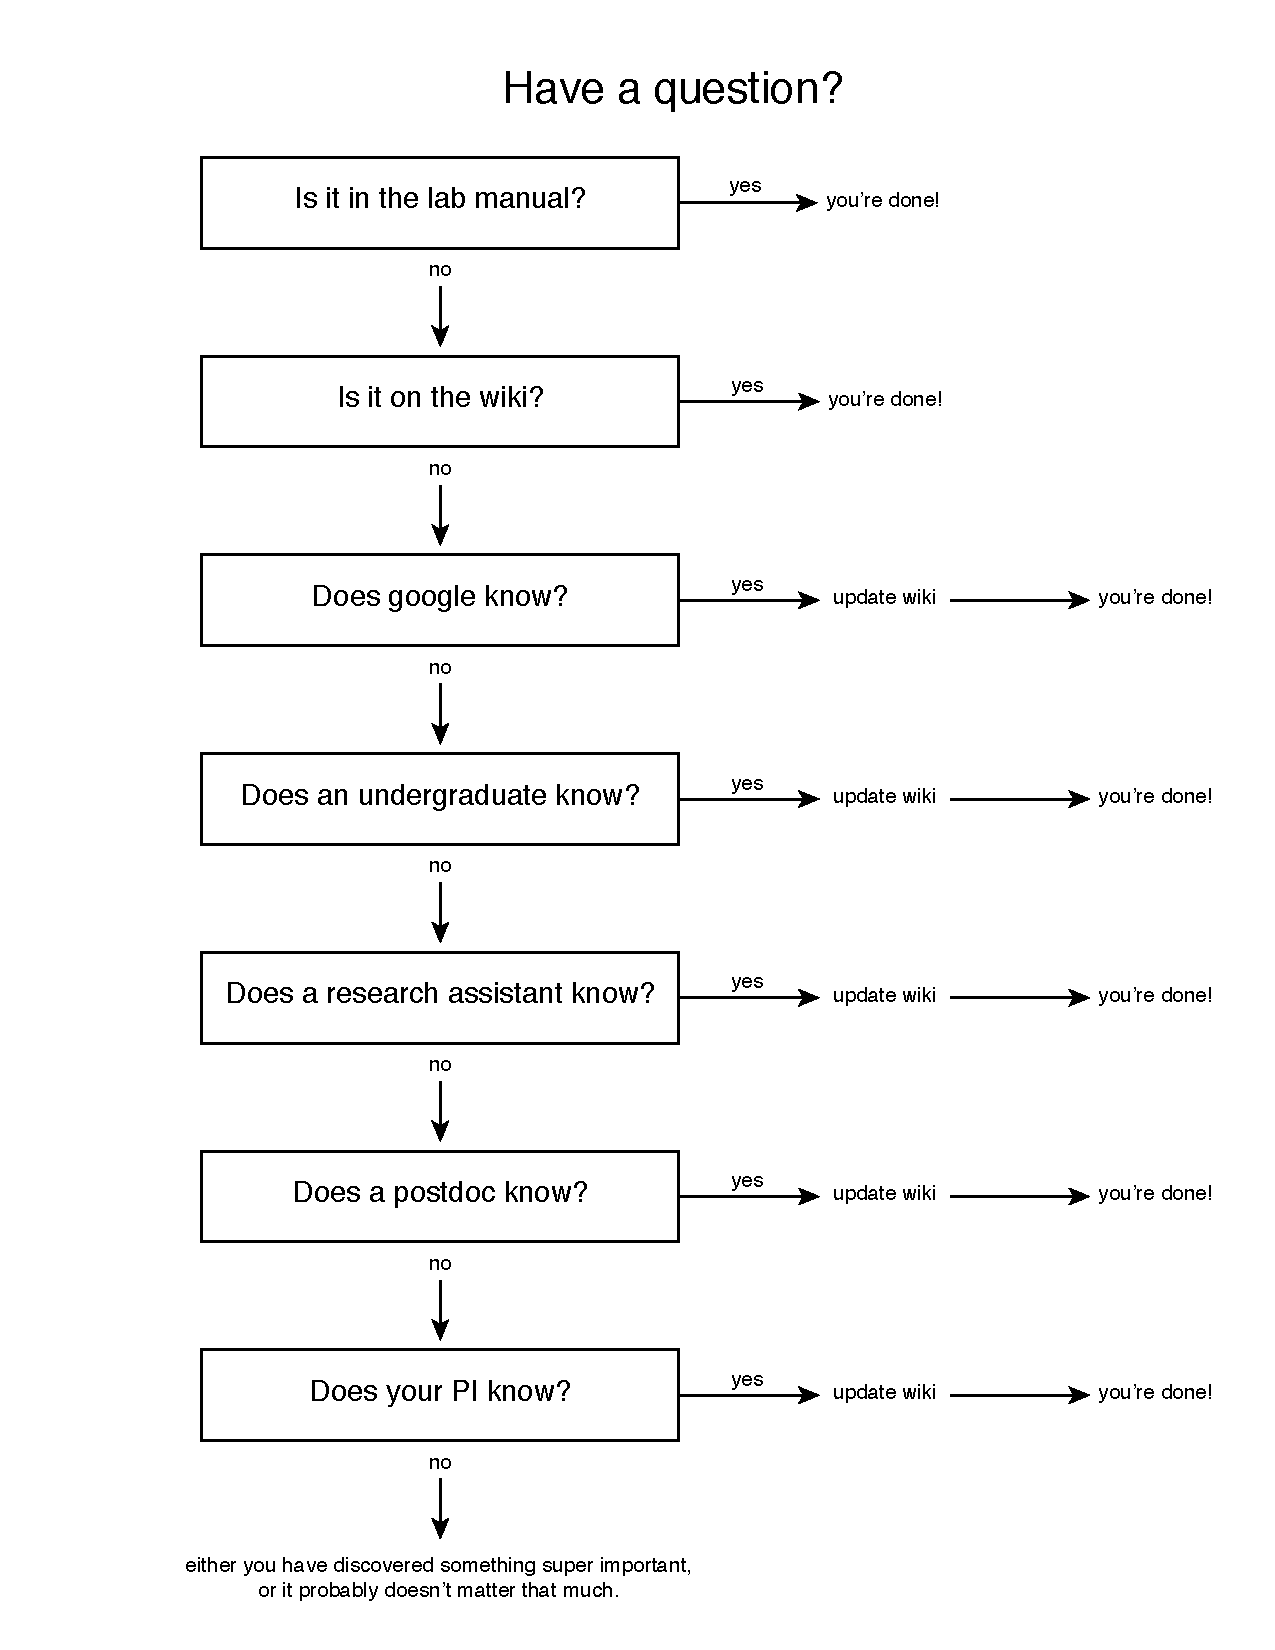
\includegraphics[width=\textwidth]{figures/lab_decision_tree.pdf}
\caption{Lab decision tree. Answers to all your questions should be in the lab wiki!}
\end{figure}

\subsection{My door}
Metaphorically my door is always open, but sometimes my door is, physically, closed (or perhaps slightly cracked open). If this is the case:

\begin{itemize}
\item If we have a meeting scheduled, then please knock. Hopefully I am around.
\item If we don't have a meeting scheduled, a closed door generally means I am trying to do some writing and should not be interrupted. Of course, if it's an emergency, please knock anyway. Otherwise, please send me a direct message on Slack or try another time.
\end{itemize}

\subsection{Lab meetings}
Regular lab meetings are essential for ensuring that current projects are moving forward and that future projects are being planned carefully. Remember, the lab is basically a small business that seeks to produce high-quality publications and highly-skilled trainees---i.e., you! We also use lab meetings to discuss administrative issues (e.g., IRB modifications) and practical issues (e.g., responsible conduct of research). In some case, we may also use lab meetings for workshops that introduce or reinforce skills (e.g., a NiPype tutorial), though I recommend allocating more time for workshops. 

Our lab meetings are generally 1-1.5 hours. During that time, \textbf{we have one or two presenters who are responsible for setting the agenda and sharing materials well in advance of the meeting}: 1) at a minimum, one person leads a journal club on a recent empirical paper that is relevant to the lab; and 2) another person presents their work, a practice talk, a project proposal, a tutorial, or a general-interest topic that is worth a group discussion. Example general-interest topics might include a recent influential review paper, responsible conduct of research, professional development, or innovative research practices. Unless you have clinical duties or class conflicts, regular attendance and participation is expected of everyone, especially those of you working to make a sustained intellectual contribution to a project (see \Sref{sec:authorship} on \pref{sec:authorship}).

Since scheduling lab meetings can be tough and everyone might not be able to make it, we generally try to keep some time open on Friday afternoons for joint lab meetings with other faculty (e.g., Penn-Temple meetings). These meetings serve as a great opportunity to share your work and hear outsider perspectives on your work. 

You should treat the lab meeting (and other research meetings) like a class: \textbf{be prepared, be present, and be engaged with the discussion}. This means you should read the material beforehand and put away your laptop during the meeting. If you're scheduled to present and you need to cancel or postpone, please give the group at least 72 hours notice. 

\subsection{Individual Meetings}
You will regularly give updates on your project (and particularly preliminary results) in lab meetings and other research meetings, but it is also extremely helpful to have regular individual meetings with me\footnote{I experimented one semester with not having these individual meetings, and I learned that everything works better with them. But, I will not have these regular individual meetings with people outside the lab unless they are spending a significant fraction of their effort on a project tied to the lab. Unfortunately, there is just not enough time in the day to have regular individual meetings with everyone who might want them and doing so would detract from the time I can spend on the lab.}. You should prepare for these meetings and expect to spent 30 minutes (or longer) going through your tasks, goals, progress, and issues. We can cover a lot of ground in 30 minutes, and we should aim to use your Asana as the agenda. So, during these meetings, have your Asana open and add tasks and notes/comments as necessary. 

In general, please do not use individual meetings to discuss technical issues that would be better for a workshop. If there's a concept or technical procedure that you're struggling with (e.g., scripting first-level analyses in FSL), chances are that you are not alone and others would benefit from a workshop (or even a refresher). Discussing these types of things as a group helps us build expertise, improve our documentation, and develop mentors for the next generation of trainees who will have the same questions (see \Sref{sec:training} on \pref{sec:training}). That said, we are still a young lab, so please don't hesitate to come grab me for analysis help, post to the `troubleshooting` channel on Slack, or post to the TUBRIC Support Forums. I want to help your work move forward while also preparing you to help the next person.

\subsection{Lab Wiki}
\label{sec:wiki}
%(see \Sref{sec:wiki} on (\pref{sec:wiki})

The lab wiki is our shared collection of knowledge about how to get things done in the lab. The lab manual you are reading now is ``top down'', in that I am writing the whole thing myself. By contrast, the wiki is a shared resource to which everyone can---and should---contribute. A good rule of thumb is that if you need to figure out how to do something, someone else in the lab will someday need to do the same thing. Whenever possible please document what you figure out on the wiki, including updating old sections which may no longer be relevant. Please encourage each other (and those working with you) to do the same!

Minimally, I expect you to improve existing documentation on the wiki as needed and also maintain your own project page. Your project page will detail all of the relevant aspects of your project that would allow someone else (e.g., you in 2 years or me today) to reproduce what you are doing. You can start with our template for this, but it's very important to keep it up to date and add notes and insights and they materialize. Thus, your Slab page for your project will also serve as your shared lab notebook that will certainly help others when one of your insights comes up in one of their searches. Remember, share your knowledge and use the wiki to facilitate that process.


\subsection{Asana and Slack}
Asana and Slack are the main tools for lab communication and are preferred to email in almost every situation. Please help me by keeping these up to date! A few thoughts and tips (find more on the Lab Wiki):

\begin{itemize}
\item Asana is just a to-do list, which makes it easy to use. My advice is to keep it simple: add a task, a description, due date, and tag whoever needs to know about its status. Then work toward completing that task. Your tasks should be ``SMART'' goals, which stands for Specific, Measurable, Attainable, Relevant, and Time-based. 
\item Be realistic and flexible with due dates in task in Asana. Of course, you should try to get things done in a timely manner---while recognizing that some tasks necessarily have to be completed before other tasks---but sometimes life happens and you have to adjust.
\item With Asana, we prefer to organize based on people, rather than specific projects, even though it is often the case that two (or more) people will be working on the same project. This organization scheme is much easier for me, and it's also helpful for others to see what's on your plate. If two people are working on the same task/goal, they can both have that on their Asana page.
\item In Slack, try to avoid direct messages for project-related discussions or questions. These questions can generally be asked in an open channel that others can see. Also, when using Slack, please use threads to help keep conversations organized and avoid spamming others.
\item Use the default settings for notifications in Slack and Asana. They are defaults for a reason. But, if the extra emails clutter your Inbox, take a few minutes to set up a filter (very easy to do in Gmail).
\item Use Asana and Slack together. You can integrate them with a few simple clicks. I will often create and assign tasks directly from Slack\footnote{If you wind up with multiple Asana accounts tied to different emails, you integrate them pretty easily.}.
\end{itemize}

\begin{shaded}
\noindent I have a love-hate relationship with Slack. While I prefer it over email for lab communication and announcements, I've noticed that it can be easy for folks to miss messages, depending on their settings and individual habits. So, don't be shy about voicing your opinion about what would optimize the signal to noise ratio on each of our Slack channels. In general, using Slack---or any tool for communication---should not be a real barrier for your progress or growth.
\end{shaded}

\subsection{Email}
When contacting me, please use Asana/Slack whenever possible. I will try to reply to emails when I can but please don't use it for anything urgent if you can avoid it. If you need to reach me urgently you can call/text my cell phone, or call the lab (where someone can get in touch with me). 

I would like to use Asana/Slack as much as possible for lab communication, but sometimes I will need to email you. I expect you will read all email sent to you and respond (if a response is needed) within one business day. If you're not going to be checking email for more than a few days (for whatever reason), please consider using a vacation message so that others know you're not on email (this suggestion also applies to holidays). The same guidelines apply to me: if I don't respond to one of your messages within one business day, please feel free to follow up; and if I'm not checking email at all, I will put up a vacation message. 


\subsection{Calendars}
Accurate calendars are extremely important in managing lab space and resources. We have a Lab Attendance calendar (for noting when you're away) and a Lab Resources calendar (for resources like laptops and testing rooms). It is crucial that everyone use the calendars regularly and ensure they are accurate. Use the lab calendars and follow the instructions described on the wiki.

If you think it will be helpful, you are also welcome to share your personal calendar with me, and I will try to attend to it. However, it is generally best to use the Lab Attendance calendar to indicate when you're away or otherwise unavailable. (You may also consider using away messages on Slack.)

Of course, you should also maintain your meetings and other commitments in your own calendar. When I set up a meeting with you, you will often get a calendar invite email from Gmail. Once you click the ``yes'' button, that event is in your calendar and there will be little to no confusion about the meeting time. 


%\subsection{Cubbies}

%In the closet are trays (aka ``cubbies'') for every lab member. If you have items you want to leave in the lab (such as papers you are working on), leave them here rather than out on a table. If you need to leave something for a lab member, put it here.

%Please check your cubby when you come into the lab.


%%%%%%%%%%%%%%%%%%%%%
\section{Communication outside the lab}

Communicating to people outside the lab is extremely important: your actions reflect not only on yourself, but on the lab, the lab director, the department, and the university. This is true both for participants (who volunteer for our studies) and scientific colleagues (whose opinions have a direct impact on our success and opportunity---they are the ones reviewing our grants and papers!). It is important that every time one of us represents the lab to a high level of quality. The less experience you have, the more preparation is required. Don't skimp!

\subsection{Phone}

\begin{itemize}
\item If the phone rings in the lab, answer it: identify the lab and your name. Most calls will be from potential (or current) research participants, so it's important they view us as professional and competent. ``Smith Lab. This is [your name here]. How may I help you?'' is a great start. 
\item Check voicemail messages daily to make sure nothing important slips through.
\item If someone calls the lab and leaves a message, call them back within one business day to confirm that we received the call. If they would like to participate in a study but we can't schedule them, thank them for their interest and ask if we can contact them in the future should one come up (if you actually will). If you are not going to contact them (or they do not qualify), tell them that we are done recruiting for that study and do not have anything else available, but thank them for their interest. Refer to \Sref{sec:participants} (\pref{sec:participants}) and the lab wiki for detailed instructions on scheduling participants and general phone etiquette.

\end{itemize}


\subsection{Manuscripts}
Scientific papers are one of the principal product of the lab. Both the quantity and quality of our papers have a direct impact on the success of the lab and serve as critical way for you to showcase your talents to those outside the lab. Together, we should strive to publish and prosper. 

\subsubsection{General}
\label{sec:ms_general}
%\Sref{sec:ms_general} (\pref{sec:ms_general}

We have an obligation to communicate our findings clearly and unambiguously. However, clear and unambiguous communication can be challenging, especially when writing a manuscript. Before you sit down to write a manuscript, I expect you to be familiar with what George Gopen calls \href{https://cseweb.ucsd.edu/~swanson/papers/science-of-writing.pdf}{``Reader Expectations"}. I also expect you to be familiar with what Steven Pinker calls the \href{https://stevenpinker.com/files/pinker/files/why_academics_stink_at_writing.pdf}{``Curse of Knowledge"}. You have to put yourself in the reader's shoes and imagine that s/he does \textit{not} know what you know. In my view, understanding how to work with ``Reader Expectations" and avoid the ``Curse of Knowledge" will help you communicate your findings clearly and unambiguously\footnote{Both Pinker and Gopen have books that are in lab, so take a look at them if you want more information.}

With these principles in mind, here are some additional guidelines for drafting a manuscript in the Smith Lab:

\begin{itemize}[noitemsep,nolistsep]
\item Always start with paragraph-level outlines of each section that include the key citations and points you intend to make.
\item Make sure all authors are on board with your paragraph-level outline before developing the content further.
\item Obsess over flow, context, and structure.
\item Remember that the reader does not know what you know.
\item Always show a manuscript (or revision) to all authors before submitting it, giving them the opportunity to comment.
\item Go over page proofs carefully, including the references. There is almost always a mistake (ours, or introduced by the publisher).
\item Always give the senior author the opportunity to look at page proofs.
\end{itemize}


\subsubsection{Formatting}

When you are out in the big world on your own, you are free to format your manuscripts however you like. While you're in the Smith Lab, when sending me a draft of a manuscript, please do the following:

\begin{itemize}[noitemsep,nolistsep]
\item Include a title, or multiple options for a title, if you are unsure. 
\item Include page numbers.
\item Include the full author list starting from the first draft, which helps clarify any authorship issues or concerns early on.
\item Include placeholders for all sections (e.g., introduction, methods, results, discussion.) even if they are empty, so that we can fill them in as we go. Having placeholders also helps clarify the organization from the beginning.
\item Use styles, especially for headings. This will help organization of the manuscript and make it easy to change font and formatting if need be. (To make a heading, don't simply select the text and make it bold; select the text and then a heading style, such as ``Heading 1''.)
\item While we are sending drafts back and forth, keep the text single-spaced. If the journal requires double spacing, we can add this at the end.
\item Embed figures and tables in the body of the manuscript rather than putting at the end, or in separate files. Again, we can change this to match journal guidelines before submitting if need be.
\end{itemize}

Some of these are good practice; others are simply my own preferences. However, if you humor me in these, it will decrease my distraction when reading your writing, and ultimately enable me to be more useful.

Your papers should be free of spelling and grammatical errors. There is no shame in asking for help with this; your fellow labmates, classmates, or the writing center (\url{http://www.temple.edu/writingctr/}) are available to help. The best proofreaders will explain to you \textit{why} things need to be changed so that you learn how to be a better writer, rather than simply correcting your writing. 


\begin{shaded}
\noindent When naming files, please include your name and a version number. If you send me a file called ``Research\_Statement.docx'', it is likely to get lost---try ``Baldrick\_research\_statement\_v01.docx'' (assuming your name is Baldrick and this is the first version you are sending me). Renaming files with initials when making comments is generally helpful; I would send this file back to you named ``\ldots\_dvs.docx''. After you incorporate any changes, you can then create a new document named ``Baldrick\_research\_statement\_v02''. For more on good practices in naming files, please see this \href{http://www2.stat.duke.edu/~rcs46/lectures_2015/01-markdown-git/slides/naming-slides/naming-slides.pdf}{page}.
\end{shaded}

\subsubsection{Figures}
If we are still trying to work out what a good figure looks like, I'm happy to talk this through with you and look at rough drafts. However, if we have a good idea of what we want in the figure, please send me something as finished and polished as you can make it---this makes it easy for me to give the most helpful feedback. If you give me something that isn't your best work, I will probably just tell you things you already know.

Most figures should be vector art (saved as PDF or EPS files). Vector-based files don't suffer the artifacts and poor quality that raster-based images show when magnified. Use a graphing program (such as R, Matlab, or JASP) to export to an EPS file, and then modify that file in Adobe Illustrator or other vector-based image-editing program (e.g., Inkscape).

\begin{shaded}
\noindent Don't use Microsoft Excel or Microsoft Powerpoint for your figures! They are never the best option. If you must organize your data in Excel, that's fine, but then do plotting in a better plotting program (e.g., R, Matlab, or Python).
\end{shaded}


\subsubsection{Corresponding authorship}
On average, I am around the longest and have the best chance of having access to data, etc. To keep the rules the same for everyone I am always corresponding author for research conducted in the lab.



\subsection{Conference Presentations}
I encourage everyone in lab to seek out conferences and meetings that would be a good venue for your work (a list of possibilities can be found on the wiki). Anyone submitting an abstract for a conference, symposium, etc. should clear this with me first, and circulate to all authors at least one week before the submission deadline.

\subsubsection{Talks}
Anyone giving a talk to a non-lab audience is required to give a practice talk to the lab at least one week before the real talk. If this is your first public talk on a lab project, plan on at least two practice talks (starting at least 2 weeks before the real talk). Practice talks should be mostly finished (final slides, practiced, and the right length) so that our comments will be as helpful as possible. Schedule one or more meetings with me ahead of time to plan or go over your slides, especially if you haven't given many talks before. You should \textit{never} have to stay up late finishing a talk.

\subsubsection{Posters}
Anyone presenting a poster should circulate an initial version to all authors at least one week before the printing deadline---which can be up to a week before you plan to leave for the conference (plan accordingly). If it's your first poster, plan to present it to the lab before you print. 

Make sure to double check the poster size and orientation for the conference, and the size of the paper or canvas it will be printed on.

For many conferences, you may want to bring a sign-up sheet where people can request an emailed PDF. However, these sign-up sheets can be difficult to read, so you could also print a QR code on your poster that links to your poster and/or include an OSF link to your poster.

\begin{shaded}
\noindent Plan ahead and be prepared when it comes to conference presentations. If you're unprepared or if you're unprofessional during a conference, then I will be much less likely to send you to conferences in the future.
\end{shaded}

% \Sref{sec:participants} (\pref{sec:participants}) 

\section{Communication with everyone}
Everything we do should be sharable with other researchers and the public. I want everyone to assume that all of their notes, instructions, data, and results will be publicly-accessible in the near future (see \Sref{sec:openscience} on \pref{sec:openscience}). 

%\subsection{Open Science Framework}

We generally use the Open Science Framework (OSF) for organizing (and sharing) materials and documentation related to our projects. To be honest, we don't really have a great system worked out for this and we've been trying for a few years. At this point, it is likely something that is best done during project planning (e.g., if you are submitting a pre-registration through OSF) or right before manuscript submission (e.g., if you are using OSF to share materials or post a preprint). At the end of the day, it is easy enough to simply link your OSF project to the current \href{https://osf.io/myxet/}{Smith Lab} page to help keep everything together and easy to find when necessary. The reason we do this is simple: If someone contacts me for additional information about one of our projects, my hope is that I can easily find the correct OSF page and send them a link with everything. And in an ideal world, this OSF link will already be in your paper and nobody will ever have to request our materials. 


%%%%%%%%%%%%%%%%%%%%%
\chapter{Science}

\section{Scientific integrity}

You have a responsibility to me, the institutions that support our work, and the broader scientific community to uphold the highest standards of scientific accuracy and integrity. By being in the lab you agree to adhere to professional ethical standards. There is never an excuse for fabricating or misrepresenting data. If you have any questions, or in the unlikely event that you have concerns about a research practice you have seen in the lab, please talk to me immediately.

It is also important that you prioritize the accuracy of your work while in the lab. Unintentional errors due to inattentiveness or rushing can be extremely damaging and produce results that turn out to be incorrect. Although there is always a pressure for a high quantity of research, it is critical that everything we do is of the highest quality. Mistakes will happen, so please double-check your work frequently. In many cases, multiple people will double-check a data set or workflow to ensure no mistakes have crept in along the way.

When collecting data, please use simple checklists to ensure that everything gets done and has someone who is responsible for each specific aspect of your protocol. \textbf{You should also analyze data as soon as you collect it to ensure that it was collected properly.}


\section{Open, accurate, and reproducible science}
\label{sec:openscience}

For lab manuscripts, it can be instructive to go through a paper checklist created by Jonathan Peelle\footnote{\url{https://github.com/jpeelle/paperchecklist}} that includes sections on open science and statistics. We don't always do this prior to submission, but it can help encourage us to continually keep these issues in mind.


\subsection{Open science}

We are working towards putting all stimuli, data, and analyses online and linked to each research publication. The idea is not to simply tick a box of ``open science'', but to make these resources readable and useable for reviewers and other researchers. In service of this:

\begin{itemize}
\item All files should be named and organized according to the \href{https://bids.neuroimaging.io/}{Brain Imaging Data Structure} (BIDS) standard.
\item Items need to be documented and described. At a minimum, each collection should have a README file\footnote{\url{http://jonathanpeelle.net/making-a-readme-file}} at the top level that provides details about the item in question (such as a set of stimuli or an analysis).
\item GitHub pages should have a README.md file that describes what is in the repository. You can also use the GitHub wiki (and link to your project OSF). In all cases, make sure your documentation provides enough information for an outside reviewer/collaborator to reproduce what you did without consulting you.
\item Code should be tested, bug-free, and (helpfully) commented. For tips on documenting code, check out this recent \href{https://journals.plos.org/ploscompbiol/article?id=10.1371/journal.pcbi.1006561}{``10 Simple Rules" paper by Benjamin Lee}.
\item Links should be permanent, ideally a DOI---which we can obtain through the \href{http://help.osf.io/m/sharing/l/524208-create-dois-and-arks}{OSF}, \href{https://figshare.com/}{FigShare}, or \href{https://zenodo.org/}{Zenodo}.
\end{itemize}

In pursuit of this high level of organization and documentation, lab members will frequently be asked to review and error-check lab materials (including text lists of stimuli, code input/output, etc.). Lab members creating stimuli or conducting research projects should organize them from the outset in a way that is conducive to eventual sharing (GitHub, OSF, Jupyter notebooks, etc.).


\subsection{Accurate science}

A key part of accuracy is anticipating and avoiding problems, and creating structures in the lab that facilitate a high level of reliability.

Inspired by a blog post on reliability in the lab\footnote{\url{http://jeffrouder.blogspot.com/2015/03/is-your-lab-highly-reliable.html}} we have a page on the lab wiki for documenting problems (this page is titled ``Mistakes to Avoid''). These ``Mistakes to Avoid'' should be discussed at lab meeting to make sure none slip through the cracks. Examples of problem events include:

\begin{itemize}
\item Any of the lab computers malfunctioning
\item Any data analysis/transfer procedure not working correctly (e.g., downloading imaging data from XNAT)
\item Not being able to find the installation disc for a software program
\item Nearly running out of money to pay participants (this counts as a ``near miss'' which we also need to discuss)
\end{itemize}

As a lab member it is your responsibility to be aware of times when things don't go as planned and bring these to the attention of the rest of the group. Even better, let's all work together to find ways of preventing such occurrences in the future.


\subsection{Checklist for scientific publications}

Anyone writing a manuscript (including an honors project) should consult the Peelle Lab Paper Checklist \footnote{\url{https://github.com/jpeelle/paperchecklist/blob/master/checklist.pdf}} and discuss with me before submitting your manuscript (ideally, early on in your project!).


\section{Participants}
\label{sec:participants}

Our research is made possible by the goodwill and generosity of our research participants. We not only need people to participate in our studies, but to try hard to do their best, and potentially return for a future study. Caring for our participants is one of the most important parts of the lab and something in which every member plays a role.

The most important thing is that participants must always be confident that we are professional and treating them with respect. All of the specific advice supports these goals. In general, it is helpful to model our interactions off of other professional situations, such as a doctor's office.

For all participants:

\begin{itemize}
\item Dress professionally: No jeans, t-shirts, sweatshirts, sneakers, or sandals. When in doubt, ask! This is true for both young and older adults---dressing professionally will help undergraduate participants to take the experiment seriously.
\item Answer the phone, and return all phone calls (and emails) promptly. Tell participants who you are, and where you are calling from: ``Hello, this is [name] calling from the Smith Lab at Temple University. I am returning your call from yesterday regarding a research study.''
\item Task instructions must be extremely clear. Ensure that the participant understands that their choices have real consequences for the money they take home (i.e., their decisions must be incentive compatible). 
\item Be prepared to answer questions. If you don't know the answer, it is completely fine to ask the participant if someone else can call them back. You are then responsible for making sure this happens quickly.
\item Arrive at least 30 minutes prior to testing time to make sure equipment and paperwork are all set, and to be around in the event the participant shows up early. Everything should be set up before the participant arrives. For people coming from off campus, you should be at the designated meeting spot 15 minutes before the agreed upon time.
\end{itemize}
	
For non-students, and especially older adults, always use a title (Dr./Ms./Mr.) and a participant's last name when addressing them. If you aren't sure how to pronounce their name, ask them.

We can also help participants feel more at ease by being thoughtful about the language we use. For example, participating in a ``research study'' is more friendly than being a ``subject'' in an ``experiment'' (e.g., see Table \ref{table:terms}).

% table for research terms
\begin{table}
\centering
\caption{Terms associated with research studies}
\begin{tabular}{ll}
\toprule
Instead of saying: & Say this:\\
\midrule
experiment& study, research study\\
subject& volunteer, participant\\
test & task or screening or game \\
\bottomrule
\end{tabular}
\label{table:terms}
\end{table}

Refer to the lab wiki for specific information on recruiting, scheduling, and testing participants.


\section{Subject payment}
\label{sec:subject_payment}

We pay our subjects in pre-filled Visa debit cards. One of the lab members checks out the possible cards, and then people testing participants will take out what they need to pay the subjects. Each subject signs a payment sheet and receipt booklet to document that they got paid. Naturally, it is very important that we keep track of this money.



\section{Testing locations}
\label{sec:testing_locations}

\begin{itemize}
\item Some of our shared testing locations are shared with other researchers, so it is very important that we are good citizens when it comes to using these spaces. Being a good citizen includes scheduling the time as required, not using more than our allotted time, and leaving the room as clean as we found it (or preferably cleaner).
\item No Smith Lab equipment should be left in shared testing rooms---this includes laptop, stimulation device, etc. (It all lives in the lab.)
\item No one should test a subject without signing out the testing room.
\end{itemize}



\section{Lab notebook}
\label{sec:lab_notebook}

Anyone conducting an independent research project should have a lab notebook for keeping track of discussions, experiments, and taking notes. In practice, your Lab Notebook will probably consist of handwritten notes on a piece of paper, your comments in Asana, and your project page in Slab. At the end of the day, I don't care where you initially store your notes, but it is very important that all of your project-related notes and insights make it to your project page on the wiki. Again, this helps you effortlessly share your knowledge and insights with your lab mates (and yourself 6 months from now). 

\section{Computers and data}

\subsection{General guidelines}

\begin{itemize}
\item Testing laptops should never leave the lab except for testing. Always sign out the computer and any other equipment on the calendar.
\item Do not install extraneous software or store personal files on the computers.
\end{itemize}

\subsection{Backing up your files and data}

Always assume that as soon as you turn your back the computer on which you have been working will explode.Thinking such dire thoughts will make it easier to follow these guidelines:

\begin{itemize}
\item If you save files to the shared lab drive (the S drive), backup will automatically happen. You can also use Google Drive and their File Stream program (we have almost unlimited space on our Team Drive, though it is capped at 400K files). 
\item Data from participants is irreplaceable and should be removed from testing computers immediately following testing and onto Google Drive.
\item \textbf{Be sure to constantly push changes to scripts up to GitHub}. Your scripts and code are almost as valuable as participant data. There is no excuse for losing scripts or code, so please use GitHub for everything.
\item When working on manuscripts, be sure to use Dropbox, Google Drive, or Box so that your files are backed up and accessible anywhere.
\end{itemize}


\section{Authorship}
\label{sec:authorship}
%\Sref{sec:authorship} (\pref{sec:authorship}

Many professional associations and journals have published authorship guidelines, which are worth looking at (for example: \href{http://www.icmje.org/recommendations/browse/roles-and-responsibilities/defining-the-role-of-authors-and-contributors.html}{ICMJE}). Many of these guidelines call for a sustained intellectual contribution; and in my view, there are two key requirements to being an author:

\begin{enumerate}
\item Contribute to the intellectual scientific content of the manuscript in a meaningful way.
\item Contribute to the writing of the manuscript in a meaningful way.
\end{enumerate}

Note that ``collect data'', ``analyze data'', or ``fund the study'' aren't on the list. Those are very important parts of a paper, but do not (on their own) warrant authorship. Being an author means understanding the content and being willing to take public responsibility for the work: a large part of this concerns the theoretical motivation and implications of the research. In practice, theoretical contributions are most often made through helping with the study design, data interpretation, and discussion about a topic.

Also note that being an author on a poster (or abstract) at a scientific meeting does not automatically make you an author on the paper. The thresholds for authorship on a poster vs. a paper are very different, and I will often be much more inclusive when it comes to posters coming out of the lab\footnote{In general, anyone who has helped with data collection/analysis over the course of at least one semester may be included as authors on posters.}.

This doesn't mean that as an undergraduate student or research assistant you can't be an author on a paper. Of course, if the study goes well and you are involved, you might be. However, you will need to know enough (or learn enough) about the subject to understand what we've done, and to significantly contribute to the writing. I won't add you to a paper just because I like you and want to help you out; I {\itshape will} consider giving you the opportunity to be involved to a degree that you have earned authorship, if you are willing to take on the challenge.

Typically one person will take on the main responsibility for writing the paper, and this person will be the first author. However, as noted above, I expect all authors to contribute to the writing of the manuscript. This contribution could take the form of helping structuring arguments, identifying key citations, and developing paragraph-level outlines. Once we have clear, paragraph-level outlines, it is easier to split some of the writing responsibility (e.g., a minor author might be more able to write a specific paragraph in the Discussion, if it is more within his/her expertise).

As papers work their way through the lengthy publication process (which can be years), it is sometimes possible that authorship may change in a way that reflects the overall intellectual contribution up to publication. For instance, if you're the first author on the initial submission and then you subsequently bail and someone else does all of the work to see it published, we will need reconsider authorship order.

With respect to authorship order---and authorship more generally---it can be instructive to think of a histogram plotting the number of hours invested into making a sustained intellectual contribution. Naturally, the first author will have the largest investment. However, it is not unreasonable to see that the 2nd author is putting in at least half as much time as the 1st author. In cases where there's no clear difference between 1st and 2nd author, we can consider assigning co-first authorship (this should be a relatively rare phenomenon). Most papers coming out of the lab will have at least 3 authors and all authors will play an essential role in developing the final product.

I assume that, unless we have talked about it, I will be an author on papers coming out of the lab. This does not mean that you should add me on to papers as a courtesy; it means that I expect you to include me in the process of discussion and writing in a way that merits authorship. In other words, the same approach I take with you.

It is worth pointing out that there are many views regarding authorship, and within any view there are always borderline cases. When collaborating with other people, I tend to defer to their own lab culture. However, it's important that within our own lab, we are clear on the expectations for authorship and transparent about authorship discussions and decisions. If you ever have any questions, please come speak to me.


%%%%%%%%%%%%%%%%%%%%%
\chapter{Other Important Information}
\section{Recommendation letters}
It is part of my job (and, thankfully, quite often a pleasure) to write letters of recommendation for people in the lab. Please give me as much notice as possible, and make sure I know the deadline, format (electronic? printed?), official name of the organization, what you are applying for, and so on. Please also send along a current CV.

If you are an undergraduate, I will write your letters on my own. For more senior lab members, I will also write your letters on my own, but please send me a draft of the letter (which I will extensively modify). The first few times you do this it will probably feel awkward. However, keep in mind that your goal is to make it as easy as possible for a letter writer (in this case, me) to complete the task by the deadline and without error. Even if I re-word a lot of the letter---which I probably will---it will still have the name of what you are applying for and details regarding how long I have known you, the projects you have worked on, and so on. This is extremely helpful in jogging my memory and will give me more time to focus on saying good things about you. Don't worry about being too ``braggy''; I have no problem toning things down if need be.

Like everything else, communication is key, and when in doubt, ask!

\section{Staying on top of the literature}
\label{sec:literature}

Anyone who is trying to make a sustained intellectual contribution to a project (see \Sref{sec:authorship} on \pref{sec:authorship}) should be spending a good chunk of time each week reading and thinking about the literature tied to that project. Dozens of relevant papers come out each month, so it becomes challenging to read everything. At Temple and in the Smith Lab, we have regular discussions of journal articles. These discussions happen through our weekly lab meeting, the Neuroeconomics Journal Club, the Neuroimaging Methods Journal Club, and the Maladaptive Motivated Behavior Seminar series. Please attend these meetings and contribute to the discussions. When you're reading papers (or even just skimming abstracts), think about the following questions:

\begin{itemize}
\item Which papers are ``good" and ``bad" (and why)? This question will be hard to answer at first. That's ok. You will get better with practice. In fact, you can now target this critical thinking skill by reading journals that publish the reviewer reports alongside the paper (e.g., \textit{eLife, European Journal of Neuroscience, Nature Communications}).
\item How exactly do the papers relate to our lab in general and to your project(s) specifically?
\item How do different papers agree/disagree with each other?
\item How do the papers contribute to big-picture questions in the field? 
\item What questions do the papers create?  
\end{itemize}

There are many different strategies for staying on top of the literature. For years, I've received Table of Content (TOC) emails from various journals each time there's a new issue of the journal. Although this strategy works well for tracking new content and coming across articles you might not normally read, it is easy to neglect these TOC emails and fall behind, especially if you're overzealous and sign up for too many journals. Recently, I've started getting a lot of information from Twitter, \href{http://pubcrawler.gen.tcd.ie/}{PubCrawler} alerts, and from Google Scholar alerts for specific authors---and I share much of what I see directly to one of the `papers-*` channels on Slack (you should share what you see, too!).

But, all of these articles can really be overwhelming. So, how can you manage all of this information? Here are my recommendations:

\begin{itemize}
\item \textbf{Stay calm, and read on!} Budget time for reading papers and synthesizing information, especially when you are in the early days of exploring a new topic or question. 
\item Set up alerts for \textit{some} journal TOC emails and use PubCrawler and Google Scholar for term- or topic-specific alerts. Also follow folks on Twitter. There are lots of smart people on Twitter who act as filters and disseminate articles (and other information) that you may find useful.
\item Use reference managing software, such as Mendeley or Zotero (both are free). These programs will help you collect references, add notes, and organize them however you like. 
\item Set aside time each week to review what you've added to Mendeley or Zotero and think about how those papers fit together.
\item Force yourself to write a couple of cohesive paragraphs each month that connects the dots on some of your favorite recent papers. You should be able to use this paragraph in a future class or paper; but even if you can't immediately, you will have at least spent some time practicing your writing and getting your head around multiple papers.
\item Develop a habit of sending me a short summary of one paper each week and link it to what you read last week and what you're planning to read next week. This approach will help you remember papers and link them together, and it will also give me an opportunity to give feedback on your writing.\footnote{Stealing this general idea from Deepu Murty.}
\end{itemize}

\begin{shaded}
\noindent The bottom line is simple: You need to read a lot and be able to synthesize different pieces of information. In science, everything is connected; but in order to see those connections---or design the experiments that will create the connections---you must know the literature like the back of your hand.
\end{shaded}


\section{Learning to code}
\label{sec:coding}

Computer programming (i.e., coding) is an essential skill that all students within psychology and neuroscience should develop\footnote{\url{http://www.russpoldrack.org/2016/05/advice-for-learning-to-code-from-scratch.html}}. Being comfortable with computer programming---especially Python and Matlab---will enable you to develop your own task scripts and wrangle data. 

Yet, learning computer programming can be a challenging task. In most situations, you will not learn how to code from psychology/neuroscience classes at Temple. Instead, you will learn from online training materials, software manuals/tutorials, other trainees, and your own experiences. Having a specific problem or goal in mind (e.g., program a new task or analyze a new dataset) helps considerably.

While you're learning to code, keep the following points in mind:

\begin{itemize}

\item Be patient and persistent. No one ``gets it'' immediately, and you may have to work through several errors before arriving at a solution. 
\item Be careful and obsessive. Most coding mishaps occur because of a tiny typo. If you're careful and thorough, you will catch these mistakes and save yourself time and frustration. 
\item Understand input and output for all scripts you use.
\item Have a basic sense of how each line of code relates to other lines of code in your script. Everything is connected. 
\item Paths errors are common. Avoid them by shoring up your understanding directory structures. Every input and output file lives in a specific location that you control. 
\item Avoid staring at the same error for more than 30 minutes. If you haven't solved it in 30 minutes, switch to some other work or take a walk outside.
\item \textbf{Don't be shy about asking for help.} Other students/trainees and internet forums (e.g., NeuroStars) are great places to find help. You can also post a quick message to the `troubleshooting` channel on Slack.

\end{itemize}


\begin{shaded}
\noindent Although learning to code can be a daunting and frustrating task, it is well worth the investment. Coding is a skill that will generalize well beyond the laboratory, particularly industry positions involving data science. 
\end{shaded}




\end{document}